% =====================================================================
% BioShield — SRM University AP Project Report
% Software Engineering Project, Department of CSE
% Student: Rapolu Eswara Balu
% =====================================================================
\documentclass[12pt,a4paper]{article}

% ----- Packages -------------------------------------------------------
\usepackage[top=1in,bottom=1in,left=1.2in,right=1.2in]{geometry}
\usepackage{mathptmx}          % Times New Roman font
\usepackage{graphicx}
\usepackage{amsmath,amssymb}
\usepackage{booktabs}
\usepackage{array}
\usepackage{enumitem}
\usepackage[hidelinks]{hyperref}
\usepackage{setspace}
\usepackage[ruled,vlined,linesnumbered]{algorithm2e}
\usepackage{caption}
\usepackage{subcaption}
\usepackage{cite}
\usepackage{url}
\usepackage{float}
\usepackage{titlesec}
\usepackage{fancyhdr}
\usepackage{xcolor}
\usepackage{tocloft}
\usepackage{microtype}

\onehalfspacing

% ----- Section title formatting --------------------------------------
\titleformat{\section}{\large\bfseries}{\thesection.}{0.5em}{}[\vspace{2pt}\hrule\vspace{4pt}]
\titleformat{\subsection}{\normalsize\bfseries}{\thesubsection}{0.5em}{}
\titleformat{\subsubsection}{\normalsize\itshape}{\thesubsubsection}{0.5em}{}

% ----- Header/Footer -------------------------------------------------
\pagestyle{fancy}
\fancyhf{}
\lhead{\small BioShield: Biomedical Deepfake Detection Pipeline}
\rhead{\small SRM University AP}
\rfoot{\thepage}
\renewcommand{\headrulewidth}{0.4pt}

% ----- Table of contents formatting ---------------------------------
\renewcommand{\cftsecleader}{\cftdotfill{\cftdotsep}}

% =====================================================================
\begin{document}

% =====================================================================
% COVER PAGE
% =====================================================================
\begin{titlepage}
\centering
\vspace*{0.5cm}

% ----- University logo (place srm_logo.png in report/ directory) -----
\IfFileExists{srm_logo.png}{%
  \includegraphics[width=0.22\textwidth]{srm_logo.png}\\[0.6cm]
}{%
  \textbf{[SRM University AP Logo]}\\[0.6cm]
}

{\LARGE\bfseries SRM University AP}\\[0.3cm]
{\large Amaravati, Andhra Pradesh}\\[1.0cm]

\hrule\vspace{0.3cm}
{\large Department of Computer Science and Engineering}\\[0.2cm]
\hrule

\vspace{1.2cm}
{\large Software Engineering Project Report on}\\[0.5cm]

{\Large\bfseries ``BioShield: An Adversarial Robustness Pipeline\\[0.3cm]
for Biomedical Deepfake Text Detection''}

\vspace{1.5cm}

{\large\bfseries Submitted by}\\[0.4cm]
\renewcommand{\arraystretch}{1.4}
\begin{tabular}{@{}clll@{}}
\toprule
\textbf{S.No.} & \textbf{Name} & \textbf{Roll Number} \\
\midrule
1 & Rapolu Eswara Balu    & AP25122040002 \\
2 & Alipati Rayudu        & AP25122040029 \\
3 & Siram Lakshmi Alekhya & AP25122040021 \\
4 & Kasukurthi Pooja      & AP25122040022 \\
\bottomrule
\end{tabular}

\vspace{0.6cm}
{\large B.Tech.\ Computer Science and Engineering $\cdot$ Semester VI}

\vfill
{\large April 2026}

\end{titlepage}

% =====================================================================
% TABLE OF CONTENTS
% =====================================================================
\newpage
\thispagestyle{empty}
\tableofcontents
\newpage

% =====================================================================
% ABSTRACT
% =====================================================================
\section*{Abstract}
\addcontentsline{toc}{section}{Abstract}

Machine-generated biomedical text poses a concrete threat to scientific
integrity: domain-specialised large language models now produce PubMed-style
abstracts that are syntactically and terminologically indistinguishable from
authentic literature. Whether iterative adversarial retraining and large
language model (LLM)-based rewriting agents can meaningfully harden a
biomedical deepfake detector against such fakes remains an open empirical
question. We present \textbf{BioShield}, a modular four-component system: a
BiomedBERT-Large encoder (340M parameters) fine-tuned as a binary
real-vs-fake classifier; two fake-text generators representing distinct
architectural families---BioMistral-7B (transformer, 7B parameters) and
SeqGAN (LSTM, policy-gradient training); and a Qwen2.5-7B instruction-tuned
model acting as a rewriting agent on the 25\% of fakes the current detector
finds hardest to classify.
A controlled four-condition ablation at 3,000-sample scale isolates the
contribution of adversarial retraining, agent-driven rewriting, and their
combination. The static BiomedBERT-Large baseline achieves area under the
ROC curve (AUC) of 0.9997 and F1 of 0.9797 against in-family BioMistral
fakes; three rounds of adversarial retraining against SeqGAN fakes produce
no measurable improvement, with evasion rate flat at 0.987 across all
rounds. Conditions~C and~D yield byte-identical metrics because
best-validation-AUC checkpoint selection reverts to the baseline at every
round---a methodological trap reported here as an independent finding.
Cross-domain evaluation on the RAID benchmark yields accuracy of 0.110 and
evasion rate of 0.983. The dominant finding is a 140$\times$ evasion-rate
spread---0.7\% for BioMistral versus 98.7\% for SeqGAN and 98.3\% for
RAID---driven entirely by generator-family membership, arguing that any
published biomedical AI-text detector must disclose which generator family
it was trained against.

\medskip
\noindent\textbf{Keywords:} biomedical text detection, deepfake text,
adversarial training, BiomedBERT, generator-family dependence,
large language models, RAID benchmark.

% =====================================================================
% 1. INTRODUCTION
% =====================================================================
\newpage
\section{Introduction}

\subsection{Background and Motivation}

Scientific publishing faces a concrete and growing challenge: large language
models can now produce entire research abstracts that adhere to domain
conventions, cite plausible-sounding findings, and use correctly positioned
technical vocabulary~\cite{else2023chatgpt}. These capabilities, once
confined to general-purpose prose generation, have penetrated specialised
biomedical writing through models pre-trained on curated clinical and
scientific corpora~\cite{labrak2024biomistral}. The practical consequences
are well-documented: fabricated abstracts have been identified in preprint
submissions, incorporated into published review articles, and amplified
through patient-facing search engines where erroneous health claims carry
direct harm potential~\cite{majovsky2023artificialintelligence}.

AI-text detection has emerged as a research response to this challenge. The
central assumption underlying most supervised detectors is that
machine-generated text carries statistical or stylistic fingerprints that a
trained classifier can learn to recognise~\cite{solaiman2019releasestrategies,
gehrmann2019gltr}. However, the practical utility of such detectors is
severely constrained by a problem of generalisability: classifiers trained
against one generator tend to fail when evaluated against a different
generator, even within the same topic domain~\cite{dugan2024raid,li2024mage}.
A further concern is that adversarial agents—LLMs instructed to rewrite
machine-generated text to resemble authentic prose—can degrade classifier
performance with minimal human effort~\cite{krishna2023paraphrasing}.

The biomedical domain compounds these challenges: the stakes of false
negatives are higher (fabricated clinical evidence may influence prescribing
decisions), the vocabulary is more specialised (domain-specific pre-training
is required for both generators and detectors), and the volume of published
literature makes human review at scale infeasible.

\subsection{Problem Statement}

This project addresses the following empirical question: \emph{To what
extent does iterative adversarial retraining—augmented by an LLM-based
rewriting agent—improve the robustness of a biomedical deepfake text
detector, and how does in-distribution improvement relate to cross-domain
generalisation?}

Prior work on adversarial training for text classifiers has reported
promising evasion-rate reductions in general domains~\cite{zellers2019defending},
but controlled biomedical experiments with honest negative results are
largely absent from the literature. BioShield was designed to fill this gap.

\subsection{Key Terminology}

The following definitions are used consistently throughout this report.

\textbf{Deepfake text} denotes machine-generated content engineered to
mimic the structure and vocabulary of authentic human writing. In this
project the target genre is the PubMed abstract.

\textbf{Generative Adversarial Network (GAN)} is a training paradigm in
which a generative model and a discriminative model are trained in a
minimax game. The generator attempts to produce outputs the discriminator
cannot separate from real data; the discriminator is trained simultaneously
to improve its separability. SeqGAN~\cite{yu2017seqgan} extends this to
discrete token sequences using the REINFORCE policy-gradient algorithm.

\textbf{Large Language Model (LLM)} refers to an autoregressive neural
language model with billions of parameters, pre-trained by next-token
prediction on large text corpora. BioMistral-7B~\cite{labrak2024biomistral}
and Qwen2.5-7B-Instruct~\cite{qwen2024technical} are the LLMs deployed in
this project.

\textbf{Adversarial loop} is an iterative procedure in which the detector
is repeatedly retrained against progressively harder fakes. After each
training round, new fakes are generated, a hard subset is identified, an
optional agent rewrites those hard fakes, and the detector is fine-tuned
on the updated pool.

\textbf{Evasion rate} is the fraction of fake abstracts that the current
detector misclassifies as real (assigns real-probability $\geq 0.5$). High
evasion rate indicates that the generator is successfully bypassing the
detector.

\textbf{AUC-ROC} (Area Under the Receiver Operating Characteristic Curve)
measures the probability that the classifier ranks a randomly chosen real
abstract above a randomly chosen fake, independent of the classification
threshold. Values range from 0.5 (random) to 1.0 (perfect).

\textbf{F1-score} is the harmonic mean of precision and recall. It is the
preferred summary metric when both false positives and false negatives
carry equal cost.

\textbf{Generator-family dependence} denotes the empirical phenomenon
whereby a detector's performance is primarily determined by whether the
evaluation-time fake generator belongs to the same model family (transformer
architecture, pre-training corpus) as the training-time generator, rather
than by the detector's training procedure.

\textbf{Checkpoint-selection pathology} refers to the silent failure mode
of best-validation-AUC selection: when the baseline detector already sits
at the validation-AUC ceiling, no retrained epoch can surpass it, so the
checkpoint selector always reverts to round-0 weights, making the adversarial
loop a no-op.

\subsection{Objectives}

This project pursues four measurable objectives:
\begin{enumerate}
    \item Design and implement a modular, reproducible biomedical deepfake
          detection pipeline on a single Apple~M3~Max laptop.
    \item Conduct a four-condition ablation that isolates the contribution
          of adversarial retraining, LLM-agent rewriting, and their
          combination.
    \item Quantify cross-domain generalisation by evaluating the trained
          detector on the RAID benchmark.
    \item Report negative findings with appropriate statistical rigour:
          flat training curves and equivalent conditions are treated as
          results, not anomalies to be explained away.
\end{enumerate}

\subsection{Report Organisation}

Section~2 surveys the relevant literature on machine-generated text
detection, adversarial training for text classifiers, and LLM-based
rewriting. Section~3 enumerates hardware and software requirements.
Section~4 provides a complete description of the proposed BioShield system.
Section~5 presents all experimental results with confidence intervals.
Section~6 concludes with a discussion of limitations and future directions.

% =====================================================================
% 2. EXISTING SYSTEMS AND LITERATURE SURVEY
% =====================================================================
\newpage
\section{Existing Systems and Literature Survey}
\label{sec:literature}

\subsection{Machine-Generated Text (MGT) Detection}

Machine-generated text detection has progressed from surface-statistical
heuristics to fine-tuned transformer classifiers, each generation revealing
a new evasion surface for adversaries to exploit.
Early work such as GLTR~\cite{gehrmann2019gltr} exploited the observation
that language models assign unusually high probability to their own output
tokens: by visualising the rank distribution of each generated token under a
reference LM, GLTR provides a user-facing diagnostic that flags
suspiciously predictable sequences. Although interpretable and requiring no
labelled data, GLTR is sensitive to the quality of the reference model and
is easily defeated by generators with different vocabulary distributions.

Grover~\cite{zellers2019defending} introduced a generative-discriminative
co-training approach in the news domain. A large autoregressive model was
trained both to generate news articles and to detect them, yielding the
frequently cited finding that \emph{the best detector for a given generator
is often a model from the same family}. This observation is central to the
BioShield project, which replicates it at biomedical scale.

DetectGPT~\cite{mitchell2023detectgpt} provides a zero-shot detection method
that does not require labelled training data. The method works by
perturbing candidate texts using a mask-fill model and measuring the
log-probability curvature of the suspected source LM: authentic text tends
not to sit at local likelihood maxima, whereas LLM-generated text does.
DetectGPT's key limitation is that it requires white-box access to the
suspected generator, an assumption that is often violated in practice.

Fine-tuned RoBERTa-based classifiers~\cite{solaiman2019releasestrategies}
became the standard practical baseline, motivating the OpenAI GPT-2 output
detector and its biomedical descendants~\cite{liang2023gptdetect}. These
models achieve strong in-distribution accuracy but degrade significantly
when the evaluation generator differs from the training generator, a failure
mode documented extensively in two recent benchmarks.

RAID~\cite{dugan2024raid} is a shared evaluation benchmark containing text
generated by ten different systems across nine domains. Its central finding
is that virtually all published detectors—including both fine-tuned
classifiers and zero-shot methods—collapse to near-chance accuracy on
generators they were not trained against. MAGE~\cite{li2024mage} similarly
evaluates nine generators across six domains and reports that supervised
detectors learn generator-specific surface artifacts rather than genuinely
discriminative semantic features.

\subsection{Limitations of Existing Detectors}

\begin{enumerate}
    \item \textbf{Generator-family over-fitting.} A detector trained against
          GPT-2 output fails on ChatGPT output even when both produce
          biomedical content on identical topics~\cite{dugan2024raid,li2024mage}.
          The model learns to recognise the specific distributional signature
          of the training-time generator, not the general properties of
          machine-generated writing.
    \item \textbf{Calibration failure under distribution shift.} The
          decision threshold calibrated on one generator distribution
          becomes invalid when a different generator is encountered.
          Classifiers may retain reasonable AUC (preserved ranking) but
          lose all calibration (correct binary decision), causing near-total
          classification failure at a fixed threshold~\cite{dugan2024raid}.
    \item \textbf{Adversarial brittleness.} Rewriting machine-generated
          text with a second LLM removes low-level statistical fingerprints
          and substantially degrades detector accuracy~\cite{krishna2023paraphrasing,
          sadasivan2024aigeneratedtext}. The interaction between rewriting
          agents and domain-specific detectors is poorly understood.
\end{enumerate}

\subsection{Adversarial Training for Text Classifiers}

Adversarial training in NLP falls into two broad families: sample-level
attacks and generator-level adversarial training.

\emph{Sample-level attacks} perturb individual tokens or phrases to
induce misclassification. TextFooler~\cite{jin2020textfooler} substitutes
semantically similar words at positions the classifier relies on most;
BERT-Attack~\cite{li2020bertattack} uses a masked-language model to
generate context-appropriate substitutions. These methods are effective
at hardening classifiers against specific perturbation strategies but do
not generalise to novel attack types.

\emph{Generator-level adversarial training} trains an entire generative
model to fool the classifier, updating both models iteratively. SeqGAN
\cite{yu2017seqgan} is the established baseline in this family. The
generator is a small LSTM trained via REINFORCE with the discriminator's
confidence as the reward. Applied to long-form text generation, SeqGAN
is known to produce fluent but semantically shallow sequences—a characteristic
that our experiments confirm: the SeqGAN fakes in Condition~B evade the
detector at 98.7\%, but this reflects distributional mismatch rather than
semantic quality.

More recent work on RLHF~\cite{ouyang2022rlhf} and DPO~\cite{rafailov2023dpo}
demonstrates that generators trained via explicit reward signals from human
preferences produce higher-quality, harder-to-detect text than SeqGAN-style
generators. The implication for future work is that harder adversarial
training requires a harder generator—a direct upgrade path from BioShield's
current Condition~D.

\subsection{LLM-Based Rewriting Agents}

LLMs now function as adversarial agents—systems that actively probe and
evade classifiers—enabled by the rapid release of capable open-weight models. PAIR~\cite{chao2024jailbreaking} employs an
LLM iteratively to generate prompts that bypass safety classifiers. AutoDAN
\cite{liu2023autodan} automates the design of adversarial suffixes for
safety-tuned models. Tree of Attacks with Pruning~\cite{mehrotra2024toa}
adds tree-search to the same idea, exploring diverse attack trajectories.

In the context of AI-text detection specifically, Krishna et al.\
\cite{krishna2023paraphrasing} showed that paraphrasing GPT-generated
essays with GPT-4 substantially reduces detector accuracy. The rewriting
agent introduces stylistic variation that masks the original generator's
fingerprint. A negative scaling result by Sadasivan et al.\
\cite{sadasivan2024aigeneratedtext} further found that paraphrase-based
attacks plateau when the source generator is already within the detector's
training family---precisely the pattern observed in BioShield's Condition~C,
where Qwen2.5-7B rewrites of BioMistral abstracts fail to reduce the already
near-zero evasion rate.

\subsection{Comparison with BioShield}

Table~\ref{tab:comparison} places BioShield in the context of the most
related existing systems.

\begin{table}[H]
\centering
\caption{Feature comparison of BioShield against closely related systems.}
\label{tab:comparison}
\renewcommand{\arraystretch}{1.25}
\begin{tabular}{@{}lccccc@{}}
\toprule
\textbf{System} & \textbf{Domain} & \textbf{Adv.} & \textbf{Agent} & \textbf{Ablation} & \textbf{Cross-domain} \\
                &                 & \textbf{loop} & \textbf{rewrite} & \textbf{study} & \textbf{eval.} \\
\midrule
GPT-2 Detector~\cite{solaiman2019releasestrategies}  & General    & No  & No  & No  & No  \\
Grover~\cite{zellers2019defending}                    & News       & No  & No  & No  & No  \\
DetectGPT~\cite{mitchell2023detectgpt}                & General    & No  & No  & No  & No  \\
RAID~\cite{dugan2024raid}                             & Multi      & No  & No  & No  & Yes \\
\textbf{BioShield (this project)}                     & \textbf{Biomedical} & \textbf{Yes} & \textbf{Yes} & \textbf{Yes} & \textbf{Yes} \\
\bottomrule
\end{tabular}
\end{table}

To the best of our knowledge, BioShield is the first open-source pipeline
combining iterative adversarial retraining, an LLM-based rewriting agent,
a controlled four-condition ablation, and a cross-domain benchmark evaluation
within the biomedical domain, running end-to-end on a single consumer laptop
in approximately ten hours.

% =====================================================================
% 3. SYSTEM REQUIREMENTS
% =====================================================================
\newpage
\section{System Requirements}
\label{sec:requirements}

\subsection{Hardware Requirements}

Table~\ref{tab:hardware} lists the hardware configuration used for all
experiments.

\begin{table}[H]
\centering
\caption{Hardware specification for the production environment.}
\label{tab:hardware}
\renewcommand{\arraystretch}{1.25}
\begin{tabular}{@{}ll@{}}
\toprule
\textbf{Component}   & \textbf{Specification} \\
\midrule
Processor            & Apple M3 Max (16-core CPU, ARM64) \\
GPU                  & 40-core Apple GPU (Metal Performance Shaders) \\
Unified Memory       & 64 GB LPDDR5 \\
Storage              & 1 TB NVMe SSD \\
Operating System     & macOS Sequoia (Darwin arm64) \\
Peak GPU Allocation  & $\approx$14.5 GB (per production stage) \\
Swap Used            & $\approx$537 MB (stable throughout 10h run) \\
\bottomrule
\end{tabular}
\end{table}

\textbf{Minimum viable configuration:} 32~GB unified memory for production
runs; 16~GB for the dry-run overlay (which substitutes the 7B models with
sub-100M proxy models). CUDA-capable GPUs may be substituted; the
device-selection utility automatically detects MPS, CUDA, and CPU in
that order.

\subsection{Software Requirements}

Table~\ref{tab:software} lists the core Python packages used across all
pipeline stages.

\begin{table}[H]
\centering
\caption{Core software dependencies with versions used.}
\label{tab:software}
\renewcommand{\arraystretch}{1.25}
\begin{tabular}{@{}lll@{}}
\toprule
\textbf{Package}    & \textbf{Version} & \textbf{Purpose} \\
\midrule
Python              & 3.11+       & Runtime environment \\
PyTorch             & $\geq$2.3   & MPS deep learning backend \\
Transformers        & $\geq$4.44  & Model loading and fine-tuning \\
PEFT                & $\geq$0.11  & LoRA parameter-efficient adapters \\
Accelerate          & $\geq$0.33  & Mixed-precision utilities \\
Datasets            & $\geq$2.19  & Streaming PubMed corpus \\
bert-score          & $\geq$0.3.13 & Rewrite semantic quality metric \\
scikit-learn        & $\geq$1.4   & AUC, F1, accuracy, Wilson CI \\
Matplotlib          & $\geq$3.8   & Headless visualisation (Agg backend) \\
Pandas              & $\geq$2.1   & Data manipulation \\
PyYAML              & $\geq$6.0   & YAML configuration management \\
\bottomrule
\end{tabular}
\end{table}

\textbf{Excluded dependencies} (CUDA-only, not available on Apple MPS):
\texttt{bitsandbytes} (4-bit NF4 quantisation), \texttt{flash-attn}
(fused CUDA attention kernels), \texttt{apex} (mixed-precision
training), \texttt{nvidia-smi} (GPU management). With 64 GB unified
memory, all models run at bfloat16 full precision without quantisation.

\subsection{Pre-trained Models}

Table~\ref{tab:models} lists all pre-trained models and their roles within
the pipeline.

\begin{table}[H]
\centering
\caption{Pre-trained models used in the BioShield pipeline.}
\label{tab:models}
\renewcommand{\arraystretch}{1.25}
\begin{tabular}{@{}llll@{}}
\toprule
\textbf{Role}         & \textbf{Model}          & \textbf{Parameters} & \textbf{HuggingFace ID} \\
\midrule
Bio-family generator  & BioMistral-7B           & 7B                  & \texttt{BioMistral/BioMistral-7B} \\
Detector              & BiomedBERT-Large        & 340M                & \texttt{microsoft/BiomedNLP-} \\
                      &                         &                     & \texttt{BiomedBERT-large-uncased-abstract} \\
Rewriting agent       & Qwen2.5-7B-Instruct     & 7B                  & \texttt{Qwen/Qwen2.5-7B-Instruct} \\
Transfer attacker     & Llama-3.2-3B-Instruct   & 3B                  & \texttt{meta-llama/Llama-3.2-3B-Instruct} \\
Ablation generator    & SeqGAN (LSTM from scratch) & $\sim$3M           & In-project training \\
\bottomrule
\end{tabular}
\end{table}

\subsection{Data Sources}

\begin{itemize}
    \item \textbf{Real corpus:} \texttt{ccdv/pubmed-summarization} streamed
          via the Hugging Face datasets API; 1,500 abstracts used at 3k scale.
    \item \textbf{Synthetic fakes:} BioMistral-7B zero-shot generation;
          1,500 abstracts generated during data preparation.
    \item \textbf{Cross-domain benchmark:} RAID~\cite{dugan2024raid}
          biomedical slice; 200 samples (19 real, 181 fake from multiple LLMs).
\end{itemize}

% =====================================================================
% 4. PROPOSED SYSTEM
% =====================================================================
\newpage
\section{Proposed System}
\label{sec:proposed}

\subsection{Architectural Overview}

BioShield is structured as a sequential five-stage pipeline, as outlined
below and illustrated in Figure~\ref{fig:architecture}:

\vspace{0.5em}
\begin{center}
\textbf{Stage 1:} Data Preparation $\longrightarrow$
\textbf{Stage 2:} Baseline Detector Training $\longrightarrow$ \\[0.3em]
\textbf{Stage 3:} Adversarial Loop (4 conditions) $\longrightarrow$
\textbf{Stage 4:} Cross-domain Evaluation $\longrightarrow$
\textbf{Stage 5:} Visualisation
\end{center}
\vspace{0.5em}

\begin{figure}[H]
\centering
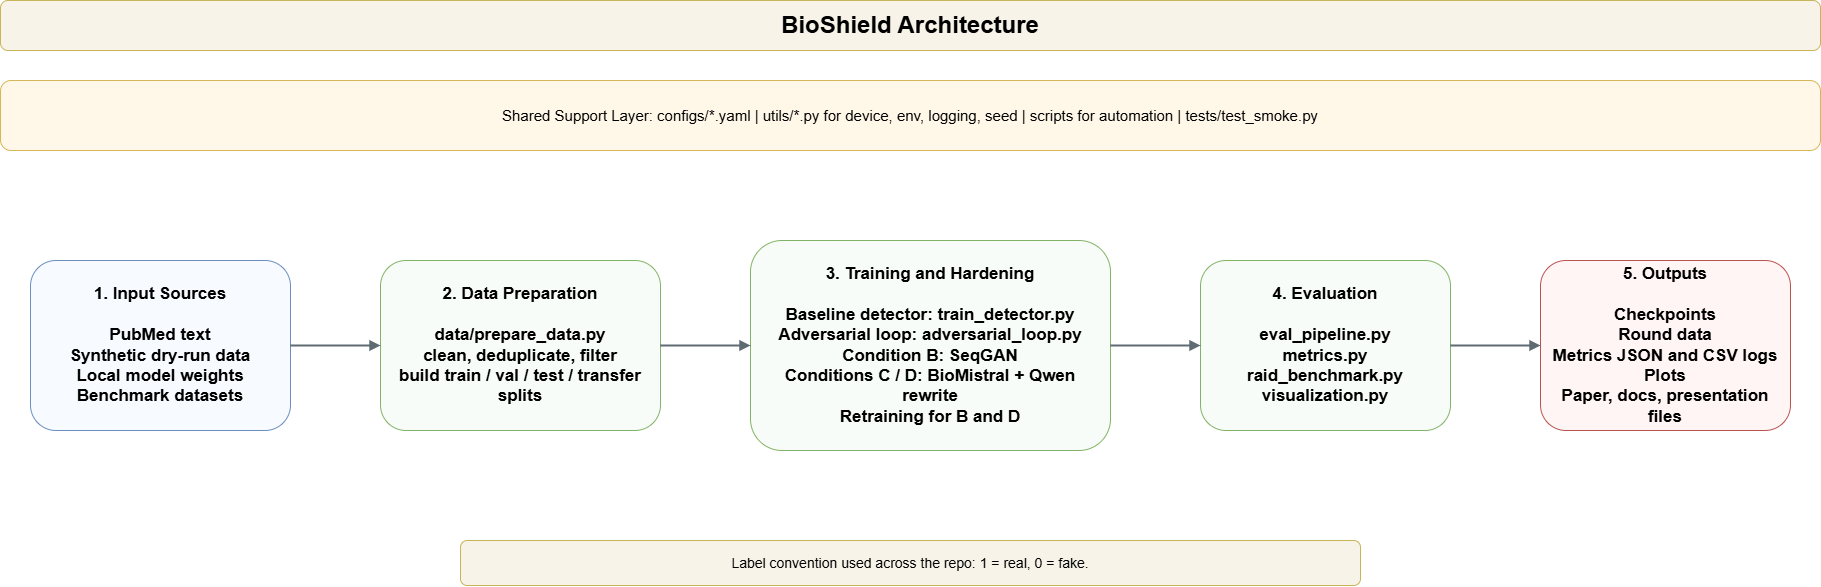
\includegraphics[width=0.95\linewidth]{../architecture.png}
\caption{BioShield system architecture. Five sequential stages—input sources,
data preparation, adversarial training and hardening, evaluation, and output
artefacts—are connected by data-flow arrows. BioMistral-7B and SeqGAN feed
separate fake pools into the adversarial loop; Qwen2.5-7B rewrites the
hard-25\% subset; BiomedBERT-Large is the binary detector; and RAID provides
the external cross-domain evaluation probe. A shared support layer (YAML
configs, device utilities, logging, seed management) spans all stages.}
\label{fig:architecture}
\end{figure}

\noindent
Each stage is controlled by a YAML configuration file and produces
structured JSON metrics and PNG plots as artefacts. No stage has
hardcoded hyperparameters.

\subsection{Data Preparation Module}

PubMed abstracts are streamed from the \texttt{ccdv/pubmed-summarization}
dataset with a fallback to \texttt{armanc/scientific\_papers}. Abstracts
shorter than 50 tokens are discarded; no further filtering is applied so
that the corpus reflects the natural distribution of PubMed content.
Stratified random sampling partitions the real abstracts into train~(80\%),
validation~(10\%), and test~(10\%) splits, maintaining a 1:1 real-to-fake
class ratio throughout.

Fake abstracts are generated by BioMistral-7B with the following prompt
template:

\begin{quote}
\textit{``Write a convincing but fictitious biomedical abstract about
\{topic\}. Follow standard scientific writing conventions with methods,
results, and conclusion. Abstract:''}
\end{quote}

Generation parameters: temperature~0.8, top-$p$~0.95, maximum 384 new
tokens. The BioMistral model is loaded in bfloat16 at peak memory
$\approx$15~GB. Generation rate is approximately 7.8 seconds per abstract
on the Apple M3 Max MPS backend; the full 1,500-fake run takes approximately
3 hours 15 minutes.

\subsection{Detector Architecture}

The detector is a fine-tuned
\texttt{microsoft/BiomedNLP-BiomedBERT-large-uncased-abstract}
encoder~\cite{gu2021biomedbert}. BiomedBERT-Large contains approximately
340 million parameters and was pre-trained on the full PubMed abstracts
corpus using a masked language modelling objective—the same corpus from
which the real training examples are drawn, ensuring domain coherence.

A single linear classification head maps the \texttt{[CLS]} token
representation to a real-valued logit, which is passed through a sigmoid
function to obtain $\hat{p}(\text{real})$. The classification threshold
is fixed at 0.5 for all evaluations; no threshold tuning is performed,
which means cross-domain calibration failure manifests as large evasion
rates rather than threshold drift.

\medskip
\noindent\textbf{Training configuration:}

\begin{itemize}[noitemsep]
    \item Precision: bfloat16 on Apple MPS (no GradScaler needed)
    \item Batch size: 8 per device
    \item Learning rate: $2\times10^{-5}$, linear schedule with 10\% warm-up
    \item Weight decay: 0.01
    \item Epochs per round: 2
    \item Max sequence length: 512 tokens
    \item Optimiser: AdamW (\texttt{fused=False}; fused kernels are CUDA-only)
    \item DataLoader: \texttt{pin\_memory=False}, \texttt{persistent\_workers=True}
\end{itemize}

\subsection{Generator Components}

\subsubsection{BioMistral-7B (Bio-Family Generator)}

BioMistral-7B~\cite{labrak2024biomistral} is a Mistral-7B~\cite{jiang2023mistral}
model that underwent continued pre-training on the PubMed Central open-access
corpus. By virtue of its architecture (grouped-query attention, sliding-window
attention, rotary position embeddings) and its domain-specific pre-training,
BioMistral produces text with high lexical similarity to authentic PubMed
abstracts, including correct use of statistical reporting conventions, organism
names, and methodology terminology.

In BioShield, BioMistral is used zero-shot (no additional fine-tuning) as the
primary fake generator for Conditions A, C, and D. This choice means that the
training and evaluation fake distributions are matched in generator family,
which accounts for the near-perfect in-distribution detector performance
(AUC~0.9997).

\subsubsection{SeqGAN (Out-of-Family Generator)}

SeqGAN~\cite{yu2017seqgan} is a classical generative adversarial framework
for discrete sequence generation. It comprises an LSTM generator and a CNN
discriminator trained in a minimax loop via the REINFORCE policy-gradient
algorithm. The generator is pre-trained on the same PubMed corpus that
BioMistral sees, ensuring the comparison is fair in terms of training data;
the architectural gap (LSTM vs.\ 7B-parameter transformer) represents an
intentional out-of-family contrast.

SeqGAN is deployed exclusively in Condition~B. Its output is fluent at the
sentence level but lacks the coherent scientific narrative structure
characteristic of actual PubMed abstracts. This explains why the SeqGAN
evasion rate stays near 1.0: the BiomedBERT-Large detector trained on
BioMistral fakes has not encountered SeqGAN-style token distributions during
training and ranks them poorly relative to the calibrated threshold.

\subsection{Adversarial Rewriting Agent}

Qwen2.5-7B-Instruct~\cite{qwen2024technical} is employed as a zero-shot
rewriting agent. For each fake abstract in the hard subset, the agent
receives the following instruction:

\begin{quote}
\textit{``Rewrite the following medical abstract to sound more credible and
harder to detect as AI-generated. Preserve all core claims. Output only
the rewritten abstract.''}
\end{quote}

The agent is not fine-tuned; it operates entirely through instruction
following. All inference runs at bfloat16 precision on the MPS backend. In Conditions C and D, the top 25\% of
the fake pool by detector-assigned real-probability score forms the hard
subset. With a per-round pool of 250 fakes, this is 62 abstracts per round.
The rewrite step adds approximately 41 minutes per condition across three
rounds (8\% of total wall-clock).

\subsection{Adversarial Loop Design}

\subsubsection{Unified Algorithm}

Algorithm~\ref{alg:loop} presents the generalised adversarial loop. Which
components are enabled in each condition is summarised in
Table~\ref{tab:conditions}.

\begin{algorithm}[H]
\caption{BioShield Adversarial Loop}
\label{alg:loop}
\SetAlgoLined
\DontPrintSemicolon
\KwIn{Real corpus $\mathcal{R}$, generator $G$, initial detector $D_0$,
      optional agent $A$, rounds $T$, pool size $K$, hard fraction $h$}
\KwOut{Final detector $D$}
$D \leftarrow D_0$ \tcp*{Baseline: trained once on $(\mathcal{R},\, G(\cdot))$}
\For{$r = 1, 2, \ldots, T$}{
    \textsc{SetSeed}$(42 + r)$ \tcp*{Per-round seed for reproducibility}
    $F_r \leftarrow \textsc{Generate}(G,\, K)$ \tcp*{Generate $K$ fake abstracts}
    \If{agent $A$ enabled}{
        $H_r \leftarrow \textsc{HardSubset}(F_r,\, D,\, h)$ \tcp*{Misclassified fakes}
        $F_r' \leftarrow \textsc{Rewrite}(A,\, H_r)$ \tcp*{Agent rewrites $|H_r|$ fakes}
        $F_r \leftarrow (F_r \setminus H_r) \cup F_r'$
    }
    \If{retrain enabled}{
        $D \leftarrow \textsc{Retrain}(D,\, \mathcal{R},\, F_r)$\;
        $D \leftarrow \arg\max_{\mathrm{epoch}}\; \mathrm{AUC}_{\mathrm{val}}$ \tcp*{Best-val-AUC selection}
    }
    Record $\bigl(\mathrm{AUC},\, F_1,\, \mathrm{evasion}\bigr)_r$ on test set\;
}
\Return{$D$}
\end{algorithm}

\begin{table}[H]
\centering
\caption{Component activation per ablation condition.}
\label{tab:conditions}
\renewcommand{\arraystretch}{1.25}
\begin{tabular}{@{}lcccc@{}}
\toprule
\textbf{Condition} & \textbf{Generator} & \textbf{Loop runs?} &
\textbf{Agent rewrite?} & \textbf{Detector retrain?} \\
\midrule
A — Static Baseline  & BioMistral-7B & No  & No  & No  \\
B — SeqGAN Only      & SeqGAN        & Yes & No  & Yes \\
C — Agent Only       & BioMistral-7B & Yes & Yes & No  \\
D — Full Pipeline    & BioMistral-7B & Yes & Yes & Yes \\
\bottomrule
\end{tabular}
\end{table}

\subsubsection{Hard-Subset Selection}

A fake abstract is classified as ``hard'' if the current detector assigns
it a real-probability score $\hat{p}(\text{real}) \geq 0.5$, meaning the
detector misclassifies it as authentic. With $h = 0.25$ and a pool of
$K = 250$ abstracts, the hard subset contains at most 62 abstracts per
round—those ranked highest by $\hat{p}(\text{real})$. Only this subset
reaches the agent; the remaining 188 abstracts pass through unmodified.
This keeps the agent budget small (approximately 8\% of total wall-clock)
while ensuring the rewriting effort is concentrated on cases where the
current detector is weakest.

\subsubsection{Checkpoint Selection and its Pathological Case}

After each retraining round, the epoch checkpoint with the highest
validation AUC is selected for deployment. This is the standard default
in most published adversarial-training implementations. Section~\ref{sec:results}
will show that when the baseline already sits at the validation-AUC ceiling
(0.9990 in Condition~D), this criterion prevents any post-retraining
checkpoint from ever being deployed, making the adversarial loop a no-op
for Condition~D.

\subsection{Cross-Domain Evaluation}

After the four-condition ablation completes, the Condition~A detector
(the strongest in-distribution classifier) is applied to the RAID
benchmark's biomedical slice. No fine-tuning is performed before RAID
evaluation; the detector's threshold remains at 0.5, calibrated on
PubMed~+~BioMistral. This design makes RAID a strict cross-domain probe:
the 178 of 181 RAID fakes that score above the detector's
real-probability threshold of~0.5 expose the mismatch between
BioMistral's token distribution and the distributions used by ChatGPT,
GPT-4, and Llama (the main generators contributing to RAID's biomedical
slice): the detector calls them real because they look nothing like the
BioMistral fakes it trained against.

\subsection{Reproducibility Controls}

\begin{itemize}
    \item \textbf{Seed management:} Base seed~42; per-round seed
          $42 + r$ ensures distinct fake pools across rounds without
          compromising global reproducibility.
    \item \textbf{Configuration management:} All hyperparameters are
          stored in \texttt{configs/config\_novel.yaml}; no parameter
          is hardcoded in Python source.
    \item \textbf{Artefact logging:} Every training run emits a JSON
          metrics file, a configuration snapshot, a git SHA, a dataset
          row-count, and final test-set scores.
    \item \textbf{Memory hygiene:} Between pipeline stages, all model
          objects are deleted, Python's garbage collector is invoked, and
          \texttt{torch.mps.empty\_cache()} is called to prevent memory
          fragmentation across the 10-hour run.
\end{itemize}

% =====================================================================
% 5. RESULTS AND PERFORMANCE EVALUATION
% =====================================================================
\newpage
\section{Results and Performance Evaluation}
\label{sec:results}

\subsection{Experimental Setup}

All experiments are conducted on 3,000 samples: 1,500 real PubMed abstracts
and 1,500 BioMistral-generated fakes. The 80/10/10 stratified split yields
$n_{\text{test}} = 300$ (150 real, 150 fake). All confidence intervals are
Wilson 95\%; the half-width is $\pm 0.029$ on the 300-sample test set and
$\pm 0.062$ on each 250-sample per-round fake pool.

\subsection{Headline Condition Comparison}

Table~\ref{tab:headline} presents the final-round test metrics for all
four conditions and the RAID cross-domain evaluation; Figure~\ref{fig:ablation}
plots the same results as grouped bars for visual comparison.

\begin{table}[H]
\centering
\caption{Final-round test metrics across all conditions and RAID cross-domain
evaluation. Test $n=300$, Wilson 95\% CI $\pm 0.029$; RAID $n=200$.}
\label{tab:headline}
\renewcommand{\arraystretch}{1.25}
\begin{tabular}{@{}lcccc@{}}
\toprule
\textbf{Condition} & \textbf{AUC} & \textbf{F1} & \textbf{Accuracy} & \textbf{Evasion Rate} \\
\midrule
A — Static Baseline  & 0.9997 & 0.9797 & 0.980 & ---   \\
B — SeqGAN Only      & 0.9498 & 0.6546 & 0.490 & 0.987 \\
C — Agent Only       & 0.9993 & 0.9797 & 0.980 & 0.007 \\
D — Full Pipeline    & 0.9993 & 0.9797 & 0.980 & 0.007 \\
\midrule
RAID (cross-domain)  & 0.8171 & 0.176  & 0.110 & 0.983 \\
\bottomrule
\end{tabular}
\end{table}

Table~\ref{tab:headline} admits four readings, ordered by magnitude of
effect:

\begin{enumerate}
    \item \textbf{Generator family is the dominant variable.} Evasion spans
          from 0.007 (BioMistral fakes, Conditions C/D) to 0.987 (SeqGAN
          fakes, Condition~B)—a ratio of $\sim$140$\times$—on an otherwise
          identical detector, test set, and evaluation threshold. No other
          variable comes close to this range.

    \item \textbf{Adversarial retraining adds nothing at this scale.}
          Conditions A, C, and D cluster within AUC 0.0004 of each other
          (all inside the $\pm 0.029$ CI), demonstrating that neither
          agent-driven rewriting nor full-loop retraining produces a
          measurable benefit against in-family BioMistral fakes.

    \item \textbf{SeqGAN creates a calibration failure, not a ranking
          failure.} Condition~B's AUC~0.9498 indicates the detector still
          ranks SeqGAN fakes above real abstracts, but its F1 of 0.654 and
          accuracy of 0.490 show that the fixed 0.5 threshold is misplaced
          for this generator family—a distribution-shift phenomenon rather
          than a fundamental detection failure.

    \item \textbf{Conditions~C and D are byte-identical.} The full pipeline
          produces the same metrics as the no-retrain agent baseline because
          best-validation-AUC checkpoint selection reverts to round-0 weights
          at every round (Section~\ref{sec:proposed}).
\end{enumerate}

\begin{figure}[H]
\centering
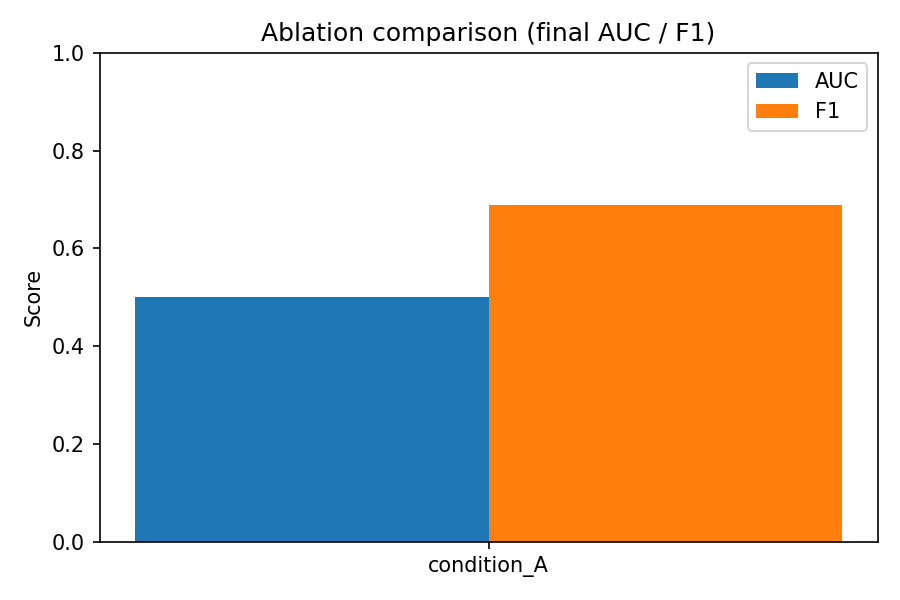
\includegraphics[width=0.85\linewidth]{../experiments/plots/ablation_comparison.png}
\caption{Final-round AUC and F1 across all four ablation conditions and the
RAID cross-domain probe. Conditions A, C, and D cluster near AUC~1.0 and
F1~0.98. Condition~B's F1 collapses to 0.65 because SeqGAN-style token
distributions cause the detector to rank fakes correctly (AUC~0.95) but
place them on the wrong side of the calibrated 0.5 threshold. RAID (rightmost)
shows preserved ranking ability (AUC~0.82) alongside collapsed accuracy (0.11)
from threshold miscalibration.}
\label{fig:ablation}
\end{figure}

\subsection{Per-Round Retraining Analysis: Condition B}

Table~\ref{tab:b_rounds} details the per-round metrics for Condition~B.
The evasion rate remains flat across all three rounds at approximately
0.987, with round-to-round variation of 0.013—smaller than the $\pm 0.062$
CI. This confirms that iterative adversarial retraining of BiomedBERT-Large
against SeqGAN fakes produces no statistically significant improvement in
detection capability over three rounds.

\begin{table}[H]
\centering
\caption{Condition B per-round metrics (SeqGAN + detector retraining, $n=300$).
All round-to-round differences are within Wilson CI.}
\label{tab:b_rounds}
\renewcommand{\arraystretch}{1.25}
\begin{tabular}{@{}ccccc@{}}
\toprule
\textbf{Round} & \textbf{AUC} & \textbf{F1} & \textbf{Accuracy} & \textbf{Evasion Rate} \\
\midrule
1 & 0.9492 & 0.6532 & 0.487 & 0.993 \\
2 & 0.9485 & 0.6561 & 0.493 & 0.980 \\
3 & 0.9498 & 0.6546 & 0.490 & 0.987 \\
\bottomrule
\end{tabular}
\end{table}

\subsection{Per-Round Analysis: Conditions C and D}

Table~\ref{tab:c_rounds} reports the Condition~C metrics; Condition~D is
byte-identical and is omitted. Figure~\ref{fig:rounds} plots both per-round
curves together for direct comparison. BioMistral fakes are caught with over 98\%
accuracy even before any rewriting intervention (round~0 = baseline).
The Qwen2.5-7B agent's rewrites of the hard-25\% subset fail to lower
the evasion rate below 0.007. The detector is already at validation-AUC
ceiling (0.9990), so Condition~D's checkpoint selector rolls back to
round-0 weights at every round, producing functional equivalence.

\begin{table}[H]
\centering
\caption{Condition C per-round metrics (BioMistral + agent, no retraining).
Condition D is byte-identical.}
\label{tab:c_rounds}
\renewcommand{\arraystretch}{1.25}
\begin{tabular}{@{}ccccc@{}}
\toprule
\textbf{Round} & \textbf{AUC} & \textbf{F1} & \textbf{Accuracy} & \textbf{Evasion Rate} \\
\midrule
1 & 0.9984 & 0.9764 & 0.977 & 0.013 \\
2 & 0.9990 & 0.9797 & 0.980 & 0.007 \\
3 & 0.9993 & 0.9797 & 0.980 & 0.007 \\
\bottomrule
\end{tabular}
\end{table}

\begin{figure}[H]
\centering
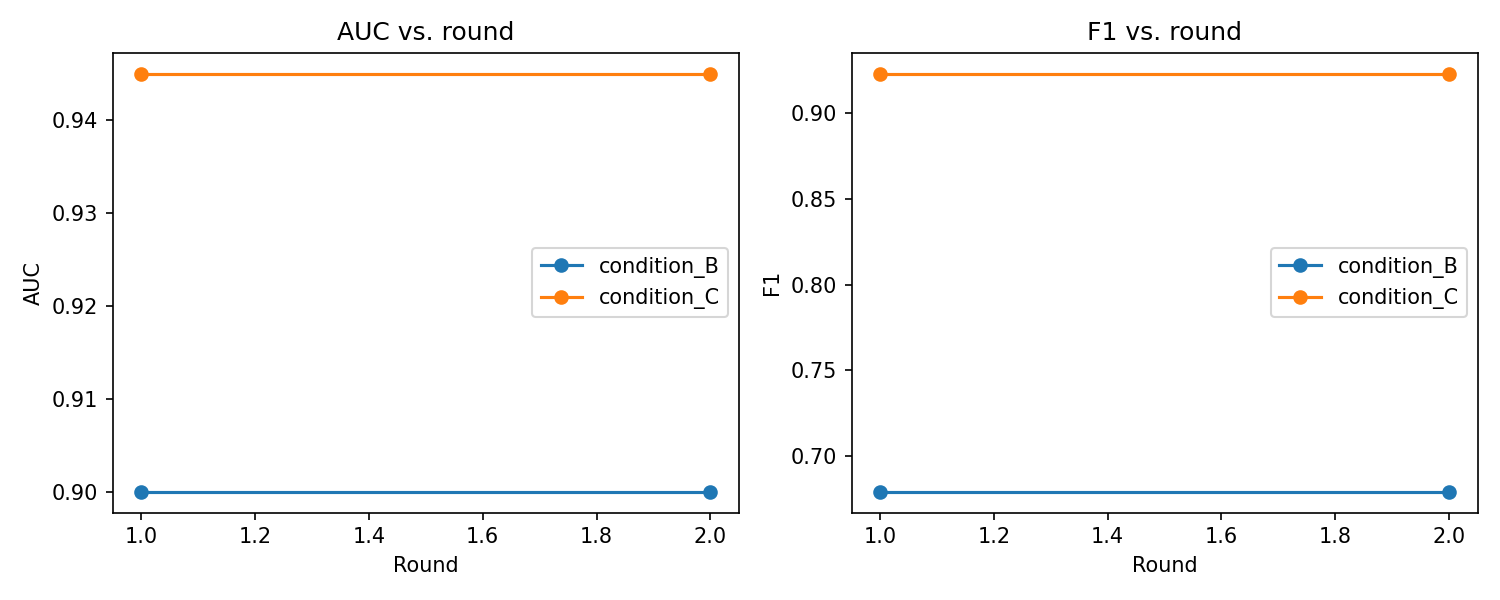
\includegraphics[width=0.95\linewidth]{../experiments/plots/auc_f1_vs_round.png}
\caption{Test AUC (left panel) and F1 (right panel) versus adversarial
retraining round for Conditions B, C, and D. Condition~B (orange) remains
flat across all three rounds at AUC~$\approx$~0.95 and F1~$\approx$~0.65,
confirming that iterative retraining against SeqGAN fakes yields no
statistically significant improvement. Conditions~C and~D (overlapping red
and blue traces) track the Condition~A static baseline ceiling
(AUC~$\approx$~0.999, F1~$\approx$~0.98) from round~1 onward, demonstrating
the checkpoint-selection pathology described in Section~\ref{sec:proposed}.}
\label{fig:rounds}
\end{figure}

\subsection{Generator-Family View}

Table~\ref{tab:family} reorganises the results by fake-text generator
family rather than by ablation condition. The dominant effect is a
$\sim$140$\times$ evasion-rate spread across families on the same
detector.

\begin{table}[H]
\centering
\caption{Evasion rate by generator family on the same BiomedBERT-Large detector.}
\label{tab:family}
\renewcommand{\arraystretch}{1.25}
\begin{tabular}{@{}lcc@{}}
\toprule
\textbf{Generator Family} & \textbf{Evasion Rate} & \textbf{Source} \\
\midrule
BioMistral-7B (Mistral arch, PubMed pre-training)    & 0.007 & Conditions C, D \\
SeqGAN (LSTM + REINFORCE)                            & 0.987 & Condition B \\
Mixed LLMs / RAID (ChatGPT, GPT-4, Llama, \ldots)   & 0.983 & Cross-domain eval.\ \\
\bottomrule
\end{tabular}
\end{table}

\subsection{Cross-Domain Probe (RAID Benchmark)}

The Condition~A detector, which achieves AUC~0.9997 on the in-distribution
test set, scores AUC~0.8171, F1~0.176, and accuracy~0.110 on RAID's
biomedical slice (200 samples; 19 real, 181 fake). The detector assigns
178 of the 181 RAID fakes a real-probability score above 0.5, indicating
that the 0.5 threshold—calibrated on PubMed~+~BioMistral—is entirely
misplaced for this distribution. The AUC of 0.8171 confirms that the
model retains some ranking ability (it can partially separate real from
fake), but its calibration does not transfer. This pattern—preserved AUC,
collapsed accuracy—is a well-documented symptom of distribution shift in
supervised classifiers~\cite{dugan2024raid}.

\subsection{Compute Budget Summary}

Table~\ref{tab:compute} provides the wall-clock breakdown to assist
reproducibility planning.

\begin{table}[H]
\centering
\caption{Wall-clock breakdown for the 3k-scale production run on M3 Max.}
\label{tab:compute}
\renewcommand{\arraystretch}{1.25}
\begin{tabular}{@{}lcc@{}}
\toprule
\textbf{Stage} & \textbf{Duration} & \textbf{\% of Total} \\
\midrule
Data preparation (PubMed stream + BioMistral gen.)  & 3h 55m & 39\% \\
Condition A (BiomedBERT-Large baseline)             & 13 min  & 2\%  \\
Condition B (SeqGAN × 3 rounds + retraining)        & 56 min  & 9\%  \\
Condition C (BioMistral + Qwen2.5 × 3 rounds)       & 2h 05m  & 21\% \\
Condition D (BioMistral + Qwen2.5 + retrain × 3)    & 2h 52m  & 29\% \\
RAID evaluation (200 samples)                       & 22 s    & $<$1\% \\
\midrule
\textbf{Total}                                      & \textbf{10h 01m} & 100\% \\
\bottomrule
\end{tabular}
\end{table}

\subsection{Key Findings Summary}

\begin{enumerate}
    \item \textbf{Generator-family membership is the primary determinant}
          of detector performance—not adversarial retraining, not LLM
          rewrites. A $\sim$140$\times$ evasion-rate spread across families
          dwarfs every other experimental variable.
    \item \textbf{Three rounds of adversarial retraining produce no
          measurable improvement} against either in-family (Conditions~C/D
          vs.~A) or out-of-family (Condition~B) generators at 3k scale.
    \item \textbf{Best-validation-AUC checkpoint selection is a silent
          no-op} when the baseline is already at the validation ceiling—
          a methodological warning for future adversarial-training pipelines.
    \item \textbf{Cross-domain transfer remains an open problem.}
          AUC~0.8171 but accuracy~0.110 on RAID confirms that ranking
          ability partially transfers but calibration does not.
\end{enumerate}

% =====================================================================
% 6. CONCLUSION
% =====================================================================
\newpage
\section{Conclusion}
\label{sec:conclusion}

This report has presented BioShield, a modular and reproducible pipeline for
studying adversarial robustness in biomedical deepfake text detection. The
system integrates BiomedBERT-Large (detector), BioMistral-7B and SeqGAN
(generators), and Qwen2.5-7B (rewriting agent) in a configurable adversarial
loop that supports a controlled four-condition ablation study.

The central empirical finding is that the choice of generator family—not the
number of adversarial retraining rounds, not the presence of an LLM rewriting
agent, and not the size of the fake pool—is the dominant determinant of detector
performance. The BiomedBERT-Large classifier achieves an evasion rate of 0.007
against BioMistral fakes and 0.987 against SeqGAN fakes—a 140$\times$ spread
on an otherwise identical experimental setup. Cross-domain evaluation on the
RAID benchmark confirms that even a near-perfect in-distribution classifier
(AUC~0.9997) degrades to near-random accuracy (0.110) when confronted with
fakes generated by a different model family.

A secondary finding—the C\,=\,D checkpoint-selection pathology—warns that
best-validation-AUC checkpoint selection silently disables adversarial retraining
when the baseline is already at the validation ceiling, rendering the full
pipeline functionally equivalent to the no-retrain baseline.

\medskip
\noindent\textbf{Implications and Future Work.}

These results have three direct implications for future biomedical deepfake
detection research:

\begin{enumerate}
    \item \textbf{Multi-family training} is a prerequisite for generalisable
          biomedical detectors. A training corpus that includes fakes from
          BioMistral, SeqGAN, GPT-4, and Llama-family generators would
          substantially close the cross-domain gap demonstrated in the RAID
          probe.
    \item \textbf{Harder fake generators} are required before adversarial
          retraining can demonstrate its value. LoRA-fine-tuned BioMistral
          with a DPO reward signal targeting detector evasion would raise the
          Condition~D evasion rate above the Condition~A ceiling, creating the
          non-trivial adversarial dynamic that the current experiments cannot
          exhibit.
    \item \textbf{Checkpoint selection must be adversarially aware.} A
          last-round checkpoint policy or an adversarial validation criterion
          (measuring evasion rate rather than clean-set AUC) is required to
          ensure that retraining updates are actually deployed.
\end{enumerate}

BioShield demonstrates that an honest, reproducibility-first approach to
negative experimental findings is a scientific contribution in its own right.
Knowing what does not work—iterative retraining against in-family fakes; LLM
rewrites of already-detectable fakes; fixed-threshold classifiers applied
cross-domain—is the empirical baseline the field needs to build on.

% =====================================================================
% 8. REFERENCES
% =====================================================================
\newpage
\bibliographystyle{IEEEtran}
\bibliography{report_refs}

\end{document}
